\RequirePackage[l2tabu, orthodox]{nag}

\documentclass[12pt, a4paper]{article}

\usepackage[english]{babel}       % Voor nederlandstalige hyphenatie (woordsplitsing)

\usepackage{amsmath}                    % Uitgebreide wiskundige mogelijkheden
\usepackage{amssymb}                    % Voor speciale symbolen zoals de verzameling Z, R...

\usepackage{microtype}

\usepackage[super]{nth}

\usepackage{booktabs}

\usepackage{url}                        % Om url's te verwerken
\usepackage{graphicx}                   % Om figuren te kunnen verwerken

\usepackage[utf8]{inputenc}           
\usepackage[T1]{fontenc}  

\usepackage{float}                      % Om nieuwe float environments aan te maken. Ook optie H!
\usepackage{listings}                   % Voor het weergeven van letterlijke text en codelistings
\usepackage{inconsolata}

\usepackage{caption}
\usepackage{subcaption}
\captionsetup[subfigure]{justification=centering}

\usepackage{multirow}

\lstset{
  belowcaptionskip=1\baselineskip,
  breaklines=true,
  frame=L,
  xleftmargin=\parindent,
  language=Lisp,
  showstringspaces=false,
  basicstyle=\footnotesize\ttfamily,
  keywordstyle=\bfseries,
  commentstyle=\itshape,
}

\usepackage{geometry}
\geometry{
  top=1in,     
  inner=1in,
  outer=1in,
  bottom=1in,
  headheight=3ex,
  headsep=2ex,
}

\usepackage{fancyhdr}                   % Voor fancy headers en footers.
\fancyhf{}
\fancyhead[L]{\slshape Neural Networks}
\fancyhead[R]{\slshape Tom Naessens}
\fancyfoot[C]{\thepage}

   
\setlength{\headheight}{15pt} % fixes \headheight warning

\usepackage[dutch]{varioref}
\usepackage[plainpages=false, hidelinks]{hyperref}    % Om hyperlinks te hebben in het pdfdocument. 
 
\graphicspath{{includes/}}               % De plaats waar latex zijn figuren gaat halen.

\renewcommand{\thesubsubsection}{Q.\arabic{subsubsection}}

\begin{document}
\selectlanguage{english}

\begin{titlepage}

\fontsize{12pt}{14pt}
\selectfont

\begin{center}

\includegraphics[height=3cm]{UGent}

\vspace{1.5cm}
Ghent University \\
Faculty of Engineering and Architecture \\
Knowledge Based Systems and Artificial Intelligence \\


\vspace{4.0cm}

\fontseries{bx}
\fontsize{17.28pt}{21pt}
\selectfont

\textsc{{\Large Bayesian Networks:} \\
{\large Medical Expert System}}

\fontseries{m}
\fontsize{12pt}{14pt}
\selectfont

\vspace{.6cm}

{\Large 
	Tom \textsc{Naessens} \hfill \\
} 

\vspace{.6cm}

{ \large
	\nth{2} master Computer Science Engineering
}

\vspace{0.4cm}

Friday November 21, 2014
\end{center}

\vspace{5.5cm}


\end{titlepage}

\thispagestyle{empty}


\pagestyle{fancy}

\subsection*{Disclaimer}
The seed used for the random generator was $2342$.

\section*{Answers to questions}
\subsection*{Distribution of the training, validation and test set}
\subsubsection{Display the distribution of P1, P2, P3 without normalizing the input, and explain the differences when the inputs are normalized.}
The result of both executions (with and without normalization) can be found in \ref{Q1} on page \pageref{Q1}. 

At first sight, the obtained curves are quite similar, both in form as in frequency values. The frequency of the training, validation and test set are also similar in both plots.

What however is different is the domain of the values of the first attribute, being the number of pregnancies. Without normalization, these reach from zero to sixteen. After normalization, these reach from approximately minus one to three. This normalization is the result of the \texttt{mapstd} function which maps the mean value to $0$ and the variance to $1$ for each row in the pattern set. 

The effects of this normalization will be discussed in the following question.

\begin{figure}[htbp]
		\centering
		\begin{subfigure}[b]{0.48\textwidth}
		        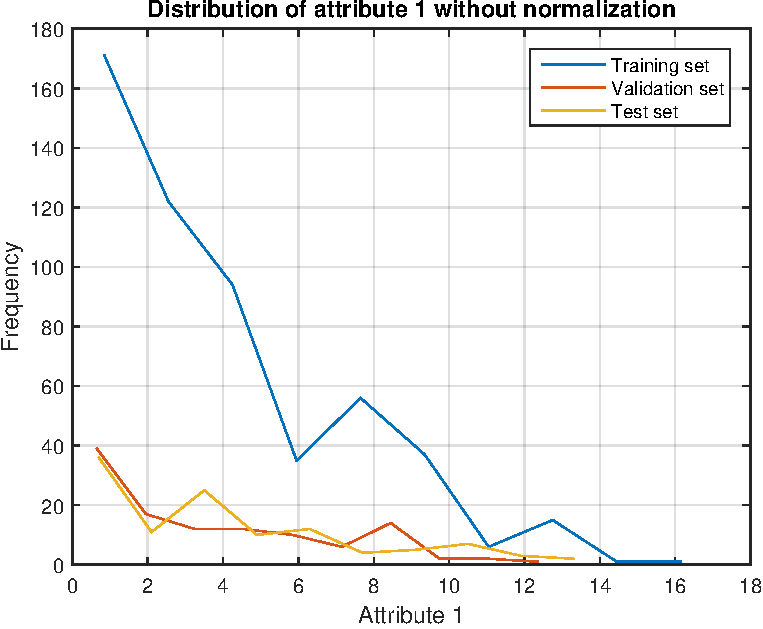
\includegraphics[width=\textwidth]{Q1}
		        \caption{Without normalization}
		\end{subfigure}
		~
		\begin{subfigure}[b]{0.48\textwidth}
		      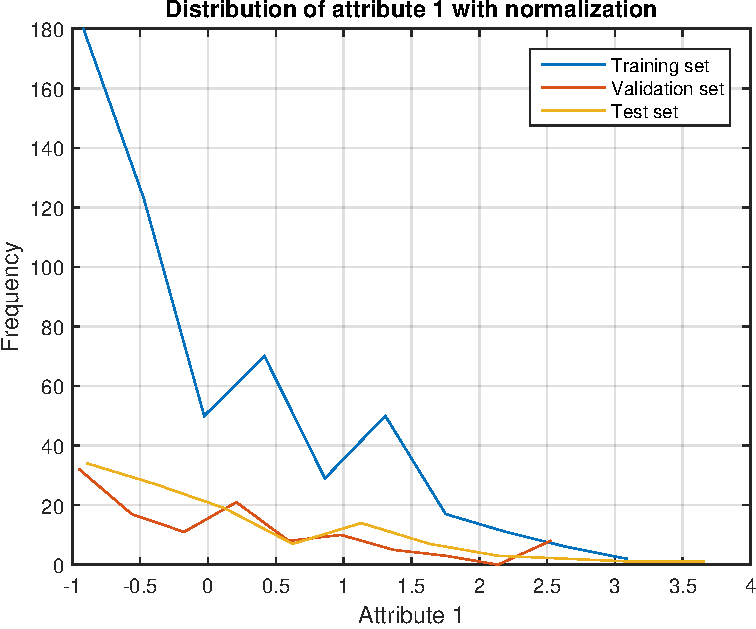
\includegraphics[width=\textwidth]{4-1-f}
		      \caption{With normalization}
		\end{subfigure}
\caption{Q.1: Distribution of P1, P2 and P3}
\label{Q1}
\end{figure}

\subsection*{Configuration and training of a neural network}
\setcounter{subsubsection}{1}
\subsubsection{Run the script without normalizing the input data. What did you determine? Explain and report the differences. Why the input normalization is recommended for any adaptive process?}
The resulting performance plots can be found in figure \ref{Q2} on page \pageref{Q2}.

There are a lot of differences we can distinct between the two plots. The first one is the course of the curves; The performances curves with normalization are a lot more ``smooth'' than the resulting curves where no normalisation was applied. The curves without normalization run in a straight line, until they drop a little bit around epoch 750. This is not the case for the performance curves with normalized data.

A second difference is the difference in validation performance. Without normalization, we obtain a performance of $0.20685$. This a lot higher than the validation performance we obtain where the data was normalized, being $0.17922$.

A third difference is found in the ``speed'' at which the an optimal performance is found for the validation set. For example, the optimum without normalization is at epoch 939 while the training with normalization reaches an optimum at epoch 538.

We can conclude that normalization benefits the training of the network in both time and performance. There are two reasons for this improvement when normalizing the input patterns:

We want the weights in the network to be tuned ``evenly'' for each input parameter in one input pattern. We don't want that very large input parameters influence the weights of the network more than smaller parameters from the same input row. By normalizing the input data for each input pattern, we mitigate this problem. 

Another reason is that, with normalization, the training does not get stuck in a local optimum as easily. Without normalization, we see that the training gets stuck from epoch 125 up till 775.

\begin{figure}[htbp]
		\centering
		\begin{subfigure}[b]{0.48\textwidth}
		        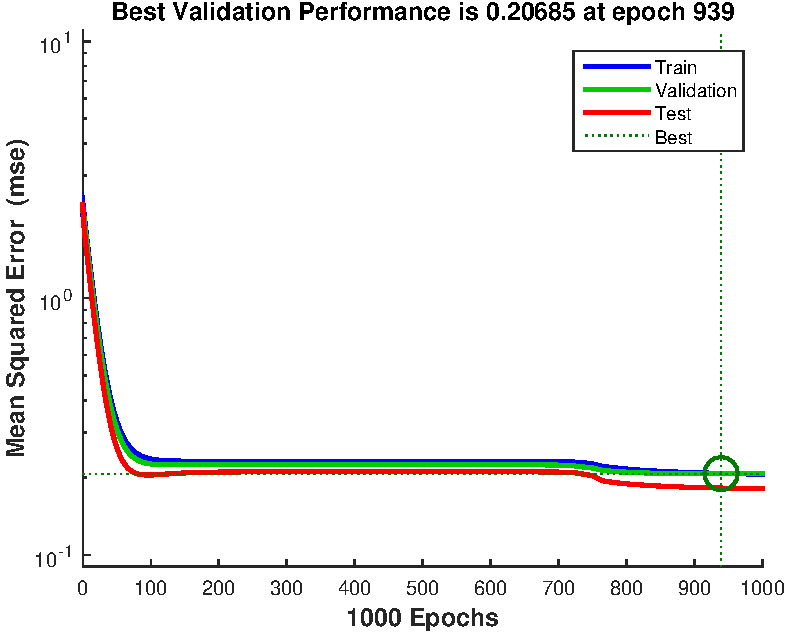
\includegraphics[width=\textwidth]{Q2-non-normalised}
		        \caption{Without normalization}
		\end{subfigure}
		~
		\begin{subfigure}[b]{0.48\textwidth}
		      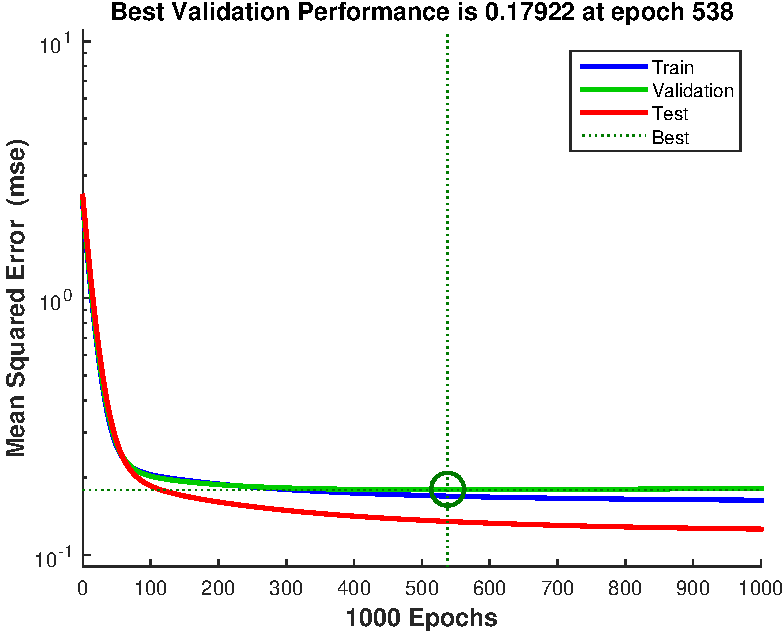
\includegraphics[width=\textwidth]{Q2-normalised}
		      \caption{With normalization}
		\end{subfigure}
\caption{Q.2: Validation performance without versus with normalization}
\label{Q2}
\end{figure}

\subsubsection{Come back to the initial configuration of the network and run the script using different learning rates (e.g. 0.5, 0.05, 0.005, 0.0005). Describe the effects on the learning curve and report them.}
The resulting performance curves for the learning are reported in figure \ref{Q3} on page \pageref{Q3}. These plots show the performance curves of the network for different learning rates, being 0.5, 0.05, 0.005 and 0.0005.

From these plots, we can see that the the faster the learning rate, the faster the curve drops. For example, in figure \ref{Q3.0005}, the curve descends slowly, while in figure \ref{Q3.5}, we see an almost vertical line followed by a horizontal line.

The effect of tthe ``speed'' of the descent is noticeable in the resulting validation performance. When the learning rate is too low, the network does may not find the optimal performance, as we can see in figure \ref{Q3.0005} where the result is 0.20494 in epoch 1000. The curves are still descending, so possibly a better solution could have been found in further iterations.

However, when the learning is too fast, some more optimal solutions could be skipped. This effect is visible in figure \ref{Q3.5} where the optimal performance is found at epoch 1000, being $0.17983$. If we compare this with plot, almost the same performance is found a lot earlier at epoch 53, or at epoch 538 in figure \ref{Q3.005}.

We can conclude that the learning rate of the network is an important parameter which needs to be selected carefully. A learning rate which is too high could cause optimums to be skipped, not to be found, or to be found at later epochs. A learning rate which is too slow could not find the optimum in time.

\begin{figure}[htbp]
		\centering
		\begin{subfigure}[b]{0.48\textwidth}
			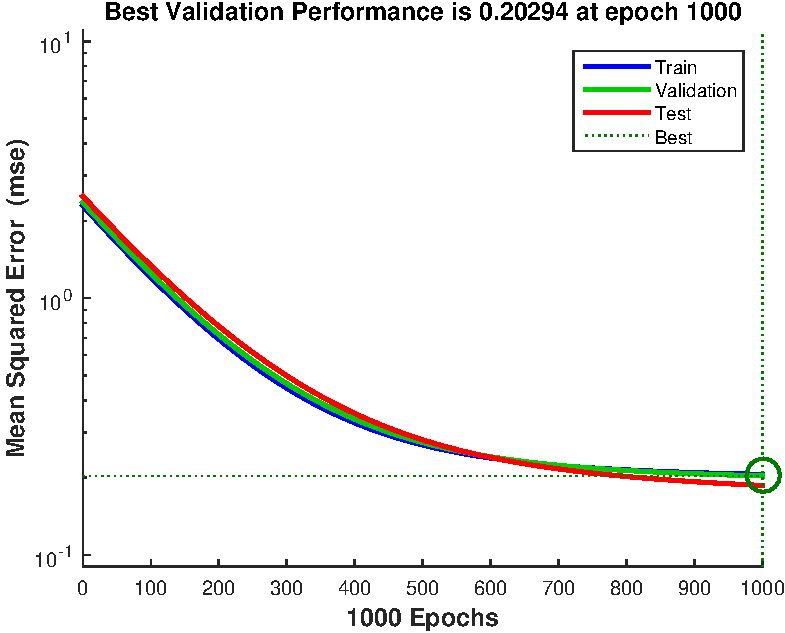
\includegraphics[width=\textwidth]{Q3-0005}
			\caption{Learning rate = 0.0005}
			\label{Q3.0005}
		\end{subfigure}
		~
		\begin{subfigure}[b]{0.48\textwidth}
			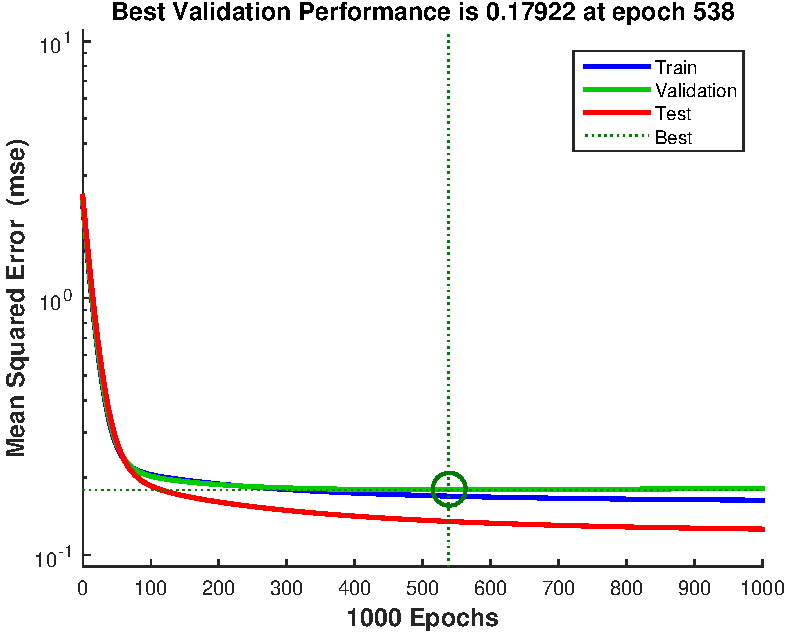
\includegraphics[width=\textwidth]{Q3-005}
			\caption{Learning rate = 0.005}
			\label{Q3.005}
		\end{subfigure}
		\\
		\begin{subfigure}[b]{0.48\textwidth}
			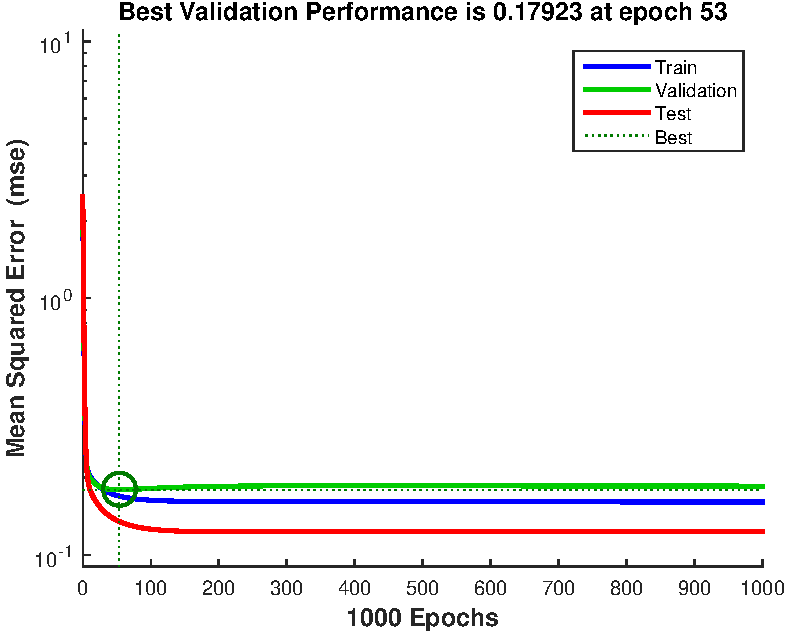
\includegraphics[width=\textwidth]{Q3-05}
			\caption{Learning rate = 0.05}
			\label{Q3.05}			
		\end{subfigure}
		~
		\begin{subfigure}[b]{0.48\textwidth}
			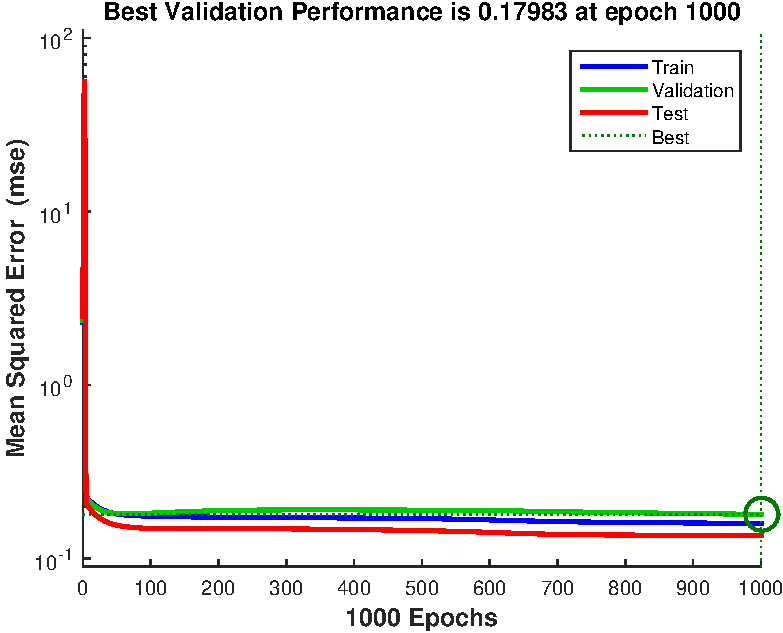
\includegraphics[width=\textwidth]{Q3-5}
			\caption{Learning rate = 0.5}
			\label{Q3.5}			
		\end{subfigure}
\caption{Q.3: Validation performance curve for different learning rates}
\label{Q3}
\end{figure}

\subsection*{Generalization versus specialization}
\setcounter{subsubsection}{3}
\subsubsection{Run the script and check the evolution of the learning curve. Note that the error of the training and validation set initially decreases, but then the error of the validation curve starts increase while training error decreases. Is the training phase experiencing generalization or specialization?}
\begin{figure}[htbp]
	\centering
	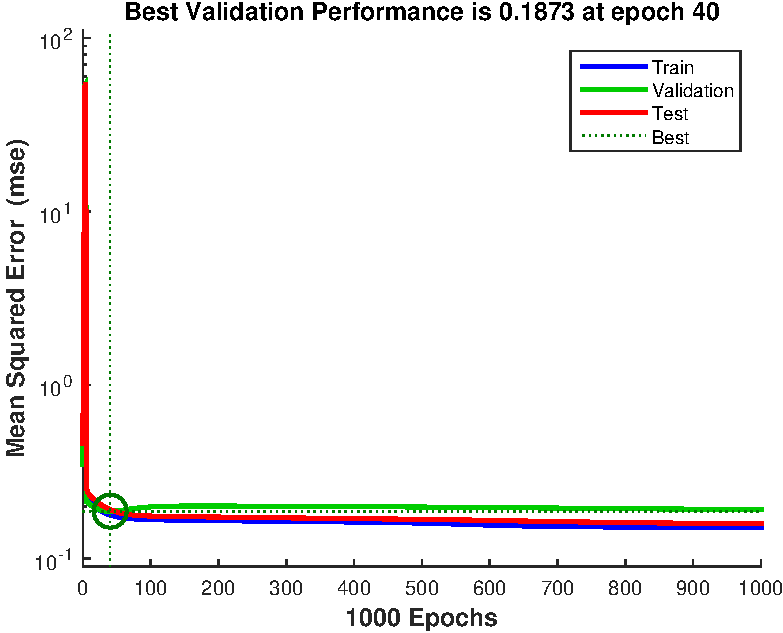
\includegraphics[width=0.6\textwidth]{Q4}
	\caption{Q4: Generalization or specialization?}
	\label{Q4}
\end{figure}
The resulting performance curve can be found in figure \ref{Q4} on page \pageref{Q4}. 

In the graph we see a clear case of overtraining or overfitting of the test set; It is indeed visible that the validation curve increased after its optimum, while the training performance still decreases. At epoch 40, the network is able to generalise the data well for data that has not been fed into the network. However, after epoch 40, the training experiences specialization and becomes less able to generalise well. We can see the effect as the validation performance error starts to increase.

\subsubsection{The data used in the previous exercise were split as follows: TRN = 70\%, VAL = 15\% and TST = 15\%. Now, run the neural network using the dividevec command using different data distributions (for example, with a relatively small amount of training data, say 5\%). What are the effects on the performance of the training, validation and test set?}
\begin{figure}[htbp]
		\centering
		\begin{subfigure}[b]{0.42\textwidth}
			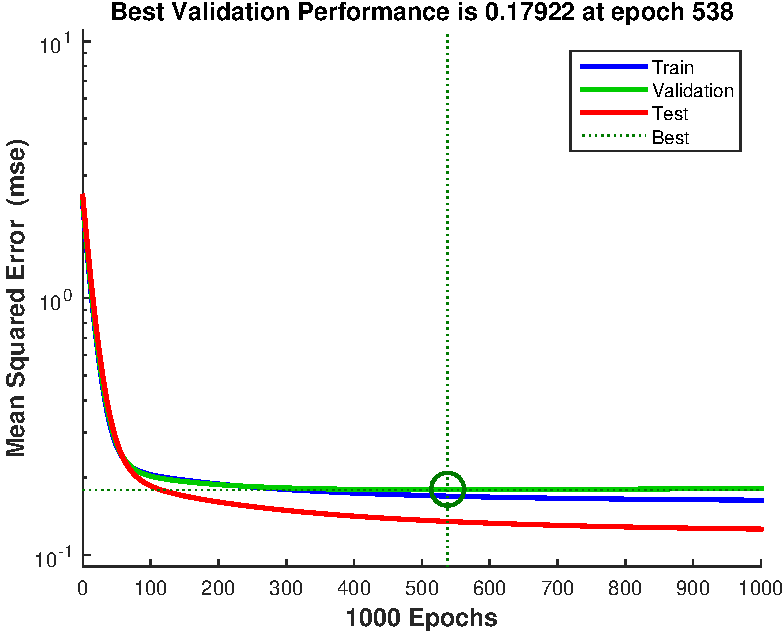
\includegraphics[width=\textwidth]{Q5-70}
			\caption{TRN=70\%, VAL=15\%, TST=15\%}
			\label{Q5-repr}
		\end{subfigure}
		~
		\begin{subfigure}[b]{0.42\textwidth}
			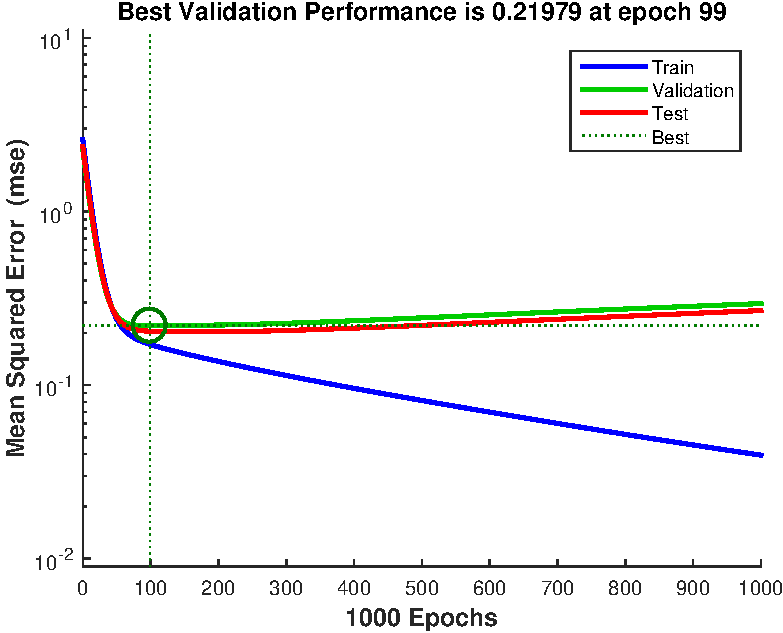
\includegraphics[width=\textwidth]{Q5-non-repr-training}
			\caption{TRN=1\%, VAL=49.5\%, TST=49.5\%}
			\label{Q5-non-repr-training}
		\end{subfigure}
		\\
		\begin{subfigure}[b]{0.42\textwidth}
			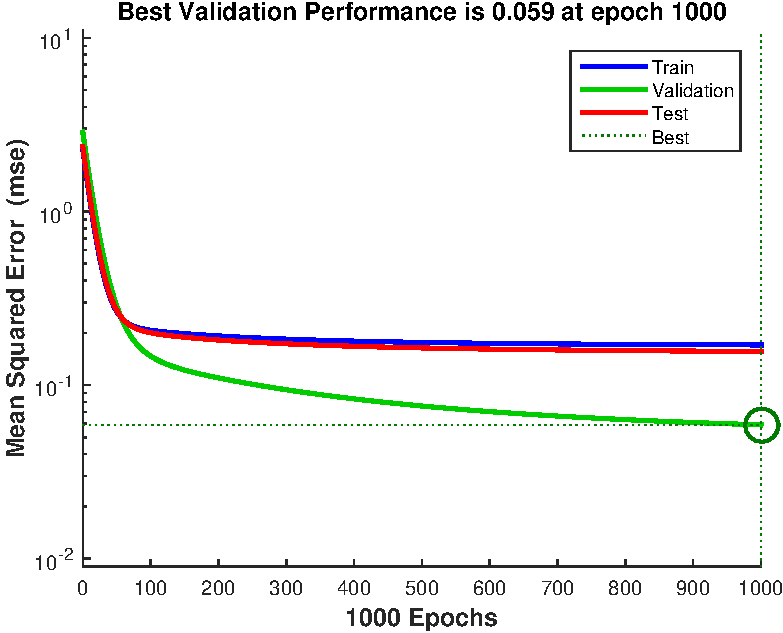
\includegraphics[width=\textwidth]{Q5-non-repr-validation}
			\caption{TRN=49.5\%, VAL=1\%, TST=49.5\%}
			\label{Q5-non-repr-validation}
		\end{subfigure}
		~
		\begin{subfigure}[b]{0.42\textwidth}
			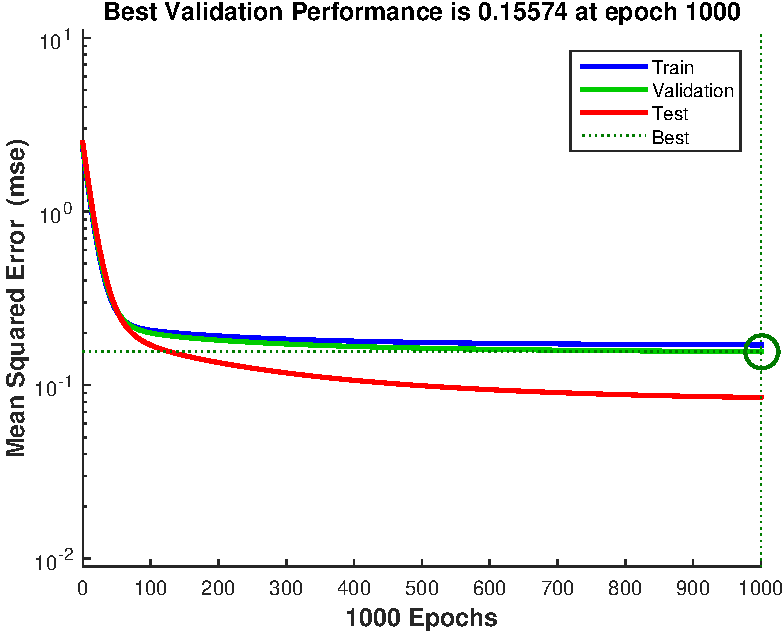
\includegraphics[width=\textwidth]{Q5-non-repr-test}
			\caption{TRN=49.5\%, VAL=49.5\%, TST=1\%}
			\label{Q5-non-repr-test}
		\end{subfigure}
	\caption{Q.5: Validation performance curve for different learning rates}
	\label{Q5}
\end{figure}

The network was tested for the ``normal'' distribution, along with three non-representative distributions. The resulting performance curves can be seen in figure \ref{Q5} on page \pageref{Q5}.

In the second curve on figure \ref{Q5-non-repr-training}, we can clearly see that the network has been trained too specific to the small set of inputs, without being able to generalise. This is clearly visible as the mean squared error of both the validation and the test set start to increase rapidly.

In the third and fourth curve on figure \ref{Q5-non-repr-validation} and \ref{Q5-non-repr-test}, we see that the validation and test curve respectively are far off from the other curves in the plot. This is simply because those distributions are not-representative. If the values in the validation or the test set were slightly different, it could well have been that the validation and/or the test curve were well above the other curves instead of below. Testing this for the same distributions, but different seeds confirms this hypothesis.

\subsection*{Influence of the number of neurons}
\setcounter{subsubsection}{5}
\subsubsection{Consider a neural network with 2 hidden layers. What is the impact on the generalization and specialization of the network by increasing the number of neurons?}

\begin{figure}[htbp]
	\centering
	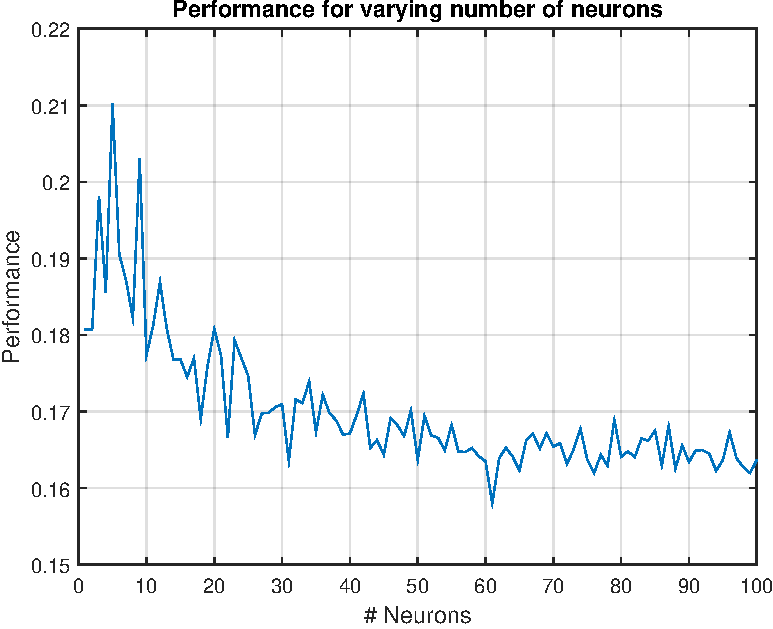
\includegraphics[width=0.6\textwidth]{Q6-100}
	\caption{Q.6: Effect of amount of neurons on the MSE}
	\label{Q6}
\end{figure}

In figure \ref{Q6} on page \pageref{Q6}, the performance for the network can be seen for 2 to 100 neurons. We can see that the performance keeps decreasing while the number of neurons increases. Running the network for 200, 500 and 1000 neurons (without plotting) confirms this hypothesis. Albeit the performance did not increase much. The time needed to run the network became increasingly longer and longer for an increasing number of neurons. Running one for 10.000 neurons for example didn't even finish in fours hours for example (after which is was cancelled).

The performance does also show some spiky behaviour. This can be attributed to the random permutation of the patterns. Sometimes, it is possible that the training and validation data differs from the test set, so a bad performance is obtained. Running the tests for 2 to 50 neurons repeatedly showed confirmed this hypothesis as the spikes lay at a different amount of neurons.

We can conclude that as the number of neurons in the network increases, the performance decreases for this set of data. It is however possible that, for other datasets, the increase in the amount of neurons would cause too much specification so the network would not generalise well for new data. This does not immediately mean that this would be the case for all networks with two hidden layers. It is perfectly possible that this neural network would not generalise well for an increasing number of neurons.

\subsubsection{What would happen if the training, validation or test set are not representative? Run the m-file with different data distributions and report your results.}

\begin{figure}[htbp]
		\centering
		\begin{subfigure}[b]{0.48\textwidth}
			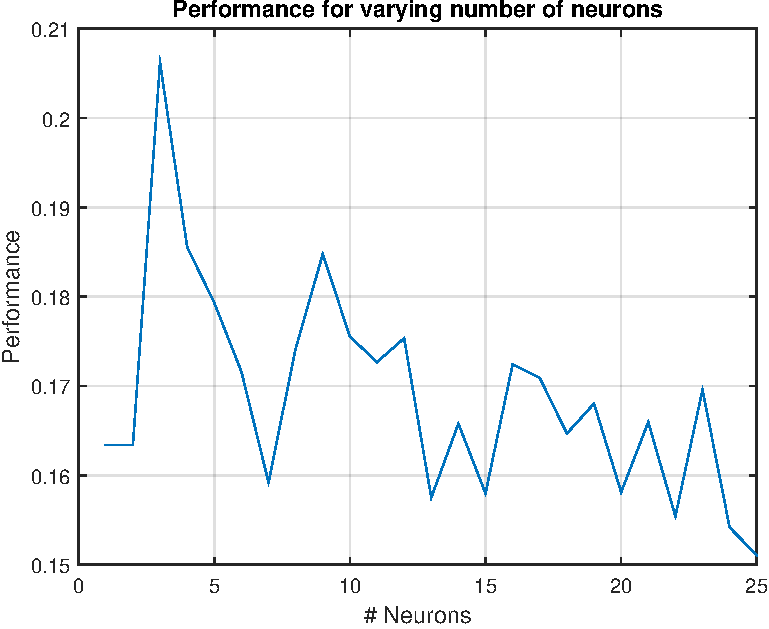
\includegraphics[width=\textwidth]{Q7-representative}
			\caption{Representative training set:\\ TRN = 40\%, VAL = 30\%, TST = 30\%}
			\label{Q7-repr}
		\end{subfigure}
		~
		\begin{subfigure}[b]{0.48\textwidth}
			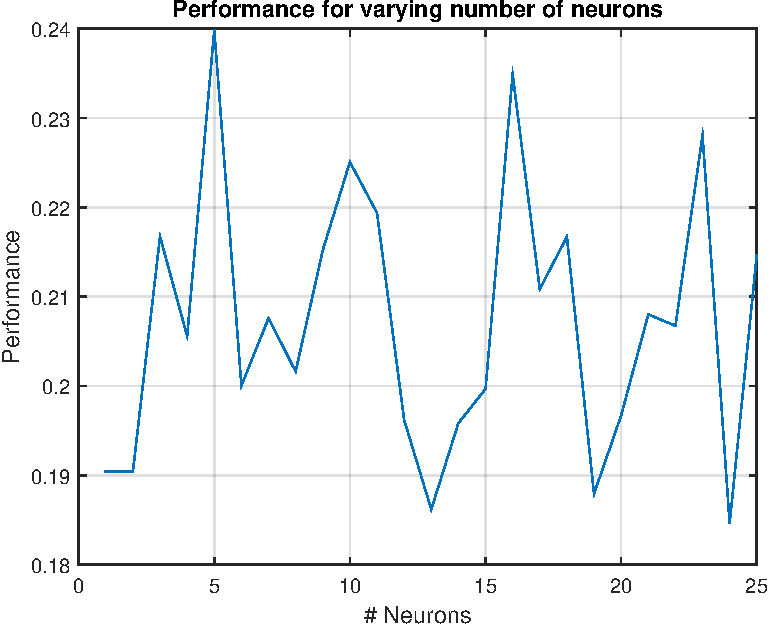
\includegraphics[width=\textwidth]{Q7-non-representative-train}
			\caption{Non-representative training set:\\ TRN = 2\%, VAL = 49\%, TST = 49\%}
			\label{Q7-non-repr-train}
		\end{subfigure}
		\\
		\begin{subfigure}[b]{0.48\textwidth}
			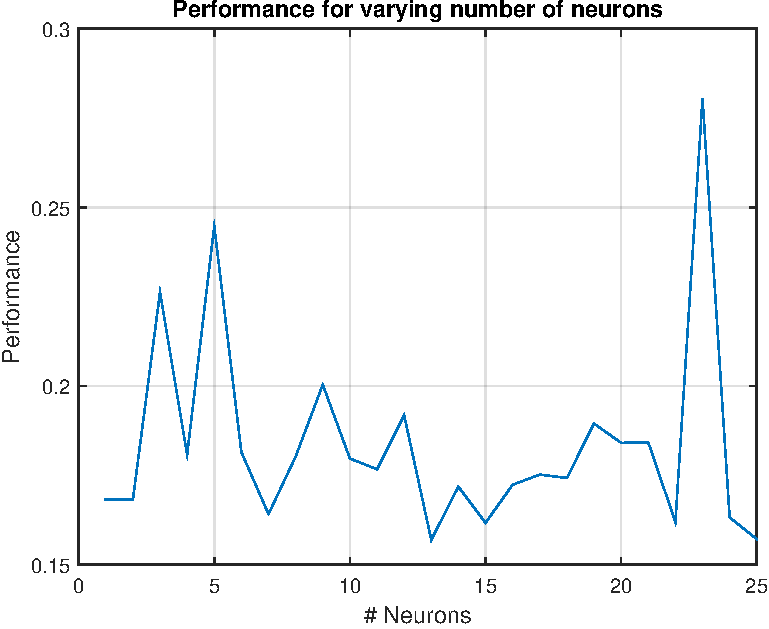
\includegraphics[width=\textwidth]{Q7-non-representative-validation}
			\caption{Non-representative validation set:\\ TRN = 49\%, VAL = 2\%, TST = 49\%}
			\label{Q7-non-repr-validation}
		\end{subfigure}
		~
		\begin{subfigure}[b]{0.48\textwidth}
			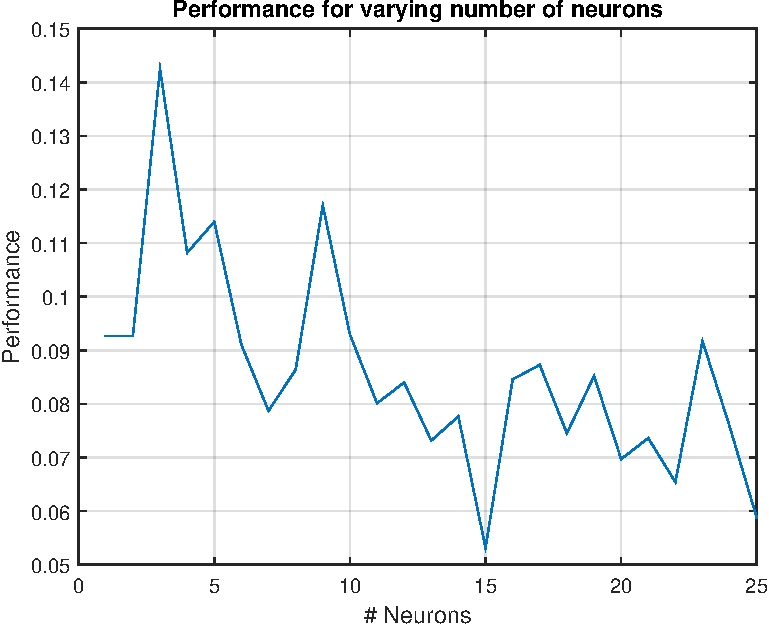
\includegraphics[width=\textwidth]{Q7-non-representative-test}
			\caption{Non-representative test set:\\ TRN = 49\%, VAL = 49\%, TST = 2\%}
			\label{Q7-non-repr-test}
		\end{subfigure}

\caption{Q.7: Effects of distribution on performance}
\label{Q7}
\end{figure}

The results for the three different non-representative distributions and a representative dataset have been plotted in figure \ref{Q7} on page \pageref{Q7}. 

When we compare the non-representative training set with the representative curves (figure \ref{Q7-repr} versus figure \ref{Q7-non-repr-train}), we see a random-looking curve for the non-representative training set, while the performance curve of the representative training set is what we would expect: a spiky but overall decreasing curve. A second difference is noticeable in the obtained performance. For (almost all) values of the amount of neurons, the obtained performance is better for the representative training set. These results we see here is because of a bias as the network did not have enough inputs be able to approach the output function closely. Not even a bigger number of neurons seems to be able to solve this problem.

When we compare the non-representative validation set with the representative curves (figure \ref{Q7-repr} versus figure \ref{Q7-non-repr-validation}), we obtain a similar result to the previous curve (figure \ref{Q7-non-repr-train}), but the differences between performances for a varying number of neurons are not as big.

When we compare the non-representative test set with the representative curves (figure \ref{Q7-repr} versus figure \ref{Q7-non-repr-test}), we see a very similar curve, which seems to perform a lot better than the curves for the representative sets. The main reason for this behaviour is that the network had more inputs to learn from, while only a very little set of inputs is being tested. If by chance (which is here the case), the patters from the test set are very similar to the test data, we obtain the impression that the network performs very well. It could also be the case that these tested input patterns were not similar to those from the input set. In this case, we would obtain a worse performance because the trained network was not able to generalize well.

\end{document}
